%HodaMahmoud
	\section{Robot Mastering}
	
	The Mastering operation calibrates the relationship between the position sensor, attached to each axis motor, and each axis angle defined for each robot. Mastering axes enables the definition of geometric parameters used to describe the analytic parameters of a robot’s geometric model. This helps in increasing the accuracy of the robot and correcting for discrepancies between design parameters and actual values.
	\newline
	Mastering the robot is performed by moving the each axis into a defined mechanical position, which is known as the “Mechanical zero position”. The zero position, which is defined by a reference notch, is an assignment to the axis drive angle. Whenever the robot moves from the mechanical zero position, its deflection represents the change in corresponding axis angle (0 increments for 0 degrees).
	\newline
	To locate the mechanical zero position of a robot axis precisely, the axes must be aligned to their pre–mastering position. The protective cap of the gauge cartridge is then removed and a dial gauge, or the supplied EMD, is fitted to it. 
	\begin{figure}[H]
        \centering
                    \textit{Note: The robot must be mastered in the same temperature conditions (either always cold or at operating temperature) to avoid inaccuracies.}
		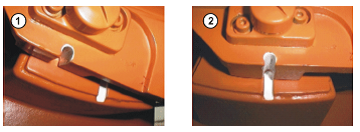
\includegraphics[scale=1.2]{mastering1}
        		\caption{Moving an axis to pre-mastering position}
    \end{figure}
    
	On passing over the reference notch, the gauge pin reaches its lowest point, the mechanical zero position is reached. The electronic measuring tool sends an electronic signal to the controller.
	
	Mastering can be performed through several methods; for older Robot versions it is performed using EMT, as for the KUKA AGILUS, mastering is done using one of these methods; EMD, dial gauge or MEMD. For our purpose, we used the MEMD supplied with the robot. The mastering positions are similar, but not identical, for all robots. Exact positions may vary between individual robots or single robot type. 
	\begin{figure}[H]
        \centering
        \textit{Note: The robot must be mastered in the same temperature conditions (either always cold or at operating temperature) to avoid inaccuracies.}
		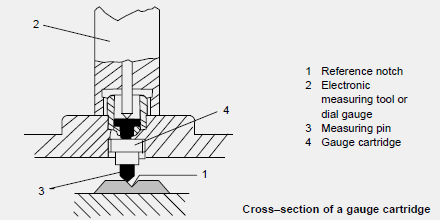
\includegraphics[scale=1]{mastering2}
		\caption{Moving an axis to pre-mastering position}
    \end{figure}
	
		\subsection{Mastering using MEMD}
		Unlike Dial gauge mastering, which requires moving the robot manually to the mastering position, MEMD mastering offers automatic movement, done by the robot, to reach the mastering position. Mastering is performed first without a load then repeated using a load. The MEMD mastering tools are shown in the below picture.
			\begin{figure}[H]
            \centering
            \textit{Note: The robot must be mastered in the same temperature conditions (either always cold or at operating temperature) to avoid inaccuracies.}
			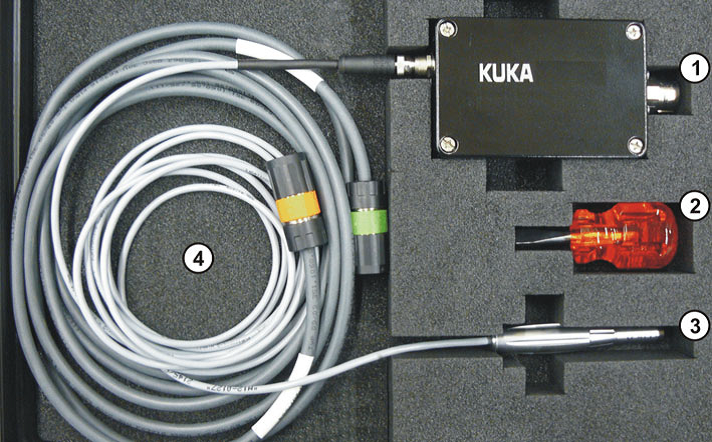
\includegraphics[scale=0.5]{mastering3}
			\caption{MEMD kit: 1. MEMD box, 2. Screwdriver, 3. MEMD, 4. Cables}
        \end{figure}
    
		\paragraph{Types of mastering}
		\begin{enumerate}
			\item First mastering (without a load).
			\item Tech offset (with a load and with saving the difference from first mastering being saved).
			\item Master load with offset is based on saving an offset value that can be used to calculate first mastering in case it was lost (used when required, carried out with a load for which an offset has already been taught. This type is used to check first mastering or to restore it in case it was lost).
		\end{enumerate}
		
		\paragraph{Precondition}
		\begin{itemize}
			\item There is no load on the robot; i.e. there is no tool, workpiece or supplementary load mounted.
			\item A1 to A5 are in the pre-mastering position.
			\item No program is selected.
			\item Operating mode T1
		\end{itemize}
		
		\paragraph{Procedure}
		\begin{enumerate}
			\item In the main menu, select Start-up > Master > EMD > With load correction > First mastering. A window opens. All axes to be mastered are displayed. The axis with the lowest number is highlighted.
			\item Remove the cover from connection X32.
			\item Connect the EtherCAT cable to X32 and to the MEMD box.
			\item Remove the protective cap of the gauge cartridge on the axis highlighted in the window.
			\item Screw the MEMD onto the gauge cartridge.
			\item Press Master.
			\item Press an enabling switch and the Start key.
			\item When the MEMD has passed through the reference notch, the mastering position is calculated. The robot stops automatically. The values are saved. The axis is no longer displayed in the window.
			\item Remove the MEMD from the gauge cartridge and replace the protective cap.
			\item Repeat steps 4 to 8 
		\end{enumerate}
	
		\paragraph{Mastering of A6}
		\begin{enumerate}
			\item Move A6 to the mastering position. A6 has very fine marks in the metal. Align these marks exactly with one another.
			\item In the main menu, select Start-up > Master > Reference.
			\item The option window Reference mastering is opened. A6 is displayed and is selected.
			\item Press Master. A6 is mastered and removed from the option window.
			\item Close the window.
			\item Disconnect the EtherCAT cable from X32 and the MEMD box.
		\end{enumerate}
		
		\fbox{\begin{minipage}{32em}
				For more information about the remaining mastering types (teach offset and mastering load with offset) and other mastering methods (using dial gauge and EMD), please refer to section “5.9 Mastering” in the provided manual “07-KSS\_82\_Software programming\_en”.
			\end{minipage}
		}
	\newpage		
	\section{Robot Calibration}
	Robot calibration is defined as identifying certain parameters in the robot’s kinematic structure, as an example; identifying relative position of robot links. Robot calibration can be performed through various methods, two of which are using a predefined and built-in calibration programs, or external methods (hardware and/or software) as RoboDK or advintec TCP. Calibration process differs in complexity from one method to another. 

	Calibration can be divided into three levels, depending on the type of modeled errors. The first of which models the differences between the actual and reported joint displacement values. This is also known as mastering. The second level, kinematic calibration, is related to the geometry of the robot and performing full geometric calibration, including angle offsets and joint lengths. The third level, non-kinematic calibration, models errors such as stiffness and friction.

	Calibration offers higher positioning accuracy for offline programmed robots. Accuracy means that the real position of the robot end effector corresponds better to the actual position calculated from the robot’s mathematical model. In the case of offline programming, pose accuracy is considered an important performance criteria.
		
	The calibration method used in out project is the first; using a predefined and built-in calibration program, which can be performed through different procedures in the KUKA platform, varying for tool and base calibration. For base calibration, these procedures are 3-point method, indirect method and Numeric input, and for tool calibration the procedures are XYZ 4-point method and XYZ reference method, both for TCP, ABC 2-point method and Numeric input. For the purpose of our project, the applied calibration procedures for both tool and base calibration were XYZ 4-point method and 3-point method respectively.

		\subsection{Tool calibration using XYZ 4-point procedure}
			The TCP of the tool to be calibrated is moved to a reference point from four different directions. The reference point can be freely selected. The robot controller calculates the TCP from the different flange positions. These four directions must be sufficiently different from one another (similar to the positions shown in the provided pictures).
            \begin{figure}[H]
                \centering
                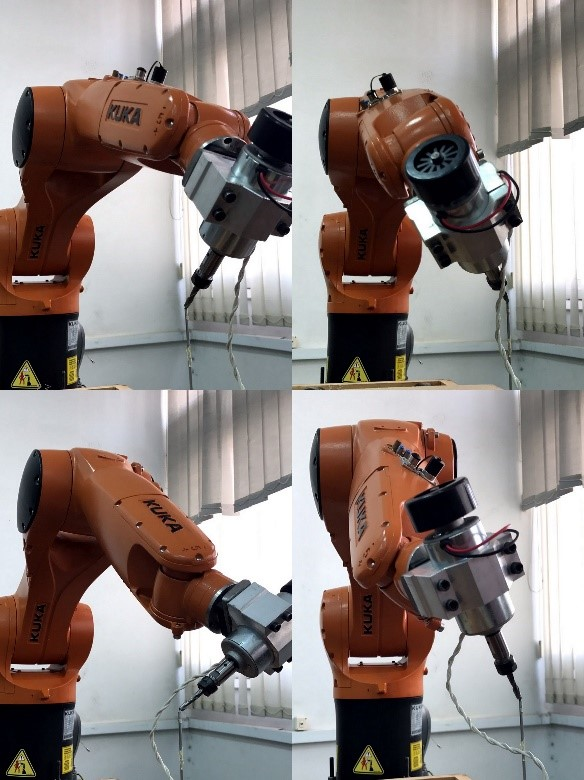
\includegraphics[width=0.7\linewidth]{calibration1}
                \caption{Tool calibration using XYZ 4-point procedure}
            \end{figure}
        
		\paragraph{Precondition}
		\begin{itemize}
			\item A previously calibrated tool is mounted on the mounting flange.
			\item Operating mode T1
		
		\end{itemize}
		
		Preparation
		
		Calculate the TCP data of the calibrated tool:
		\begin{enumerate}
			\item In the main menu, select Start-up > Calibrate > Tool > XYZ Reference.
			\item Enter the number of the calibrated tool.
			\item The tool data are displayed. Note the X, Y and Z values.
			\item Close the window.
		\end{enumerate}
		
		Procedure
		\begin{enumerate}
			\item In the main menu, select Start-up > Calibrate > Tool > XYZ Reference.
			\item Assign a number and a name for the new tool. Confirm with Next.
			\item Enter the TCP data of the calibrated tool. Confirm with Next.
			\item Move the TCP to a reference point. Press Calibrate. Answer the request for confirmation with Yes. 
			\item Move the tool away and remove it. Mount the new tool.
			\item Move the TCP of the new tool to the reference point. Press Calibrate. Answer the request for confirmation with Yes.
			\item Enter the payload data. (This step can be skipped if the payload data are entered separately instead.)
				(>>> 5.12.3 "Entering payload data" Page 138)
			\item Confirm with Next.
			\item If required, coordinates and orientation of the calibrated points can be displayed in increments and degrees (relative to the FLANGE coordinate system).
			\item For this, press Meas. points. Then return to the previous view by pressing Back.
			\item Either: press Save and then close the window via the Close icon.
			Or: press ABC 2-point or ABC World. The previous data are automatically saved and a window is opened in which the orientation of the TOOL coordinate system can be defined.
		\end{enumerate}
		
		\subsection{Base calibration using 3-point method}
		
		During base calibration, the user assigns a Cartesian coordinate system (BASE coordinate system) to a work surface or the workpiece. The BASE coordinate system has its origin at a user-defined point. In 3-point calibration, the robot moves to the origin and 2 further points of the new base. These 3 points define the new base.
		
		Advantages of base calibration
		\begin{enumerate}
			\item The TCP can be jogged along the edges of the work surface or workpiece.
			\item Points can be taught relative to the base. If it is necessary to offset the base, e.g. because the work surface has been offset, the points move with it and do not need to be retaught.
		\end{enumerate}
		
		Precondition
		\begin{itemize}
			\item A previously calibrated tool is mounted on the mounting flange.
			\item Operating mode T1
		\end{itemize}
		
		Procedure
		\begin{enumerate}
			\item In the main menu, select Start-up > Calibrate > Base > ABC 3-point.
			\item Assign a number and a name for the base. Confirm with Next.
			\item Enter the number of the mounted tool. Confirm with Next.
			\item Move the TCP to the origin of the new base. Press Calibrate. Answer the request for confirmation with Yes.
			\item Move the TCP to a point on the positive X-axis of the new base. Press Calibrate. Answer the request for confirmation with Yes.
			\item Move the TCP to a point in the XY plane with a positive Y value. Press Calibrate. Answer the request for confirmation with Yes.
			\item If required, coordinates and orientation of the calibrated points can be displayed in increments and degrees (relative to the FLANGE coordinate system). For this, press Meas. points. Then return to the previous view by pressing Back.
			\item Press Save.
		\end{enumerate}
		
			\fbox{\begin{minipage}{32em}
				For more information about tool and base calibration, please refer to section “5.11 Calibration” in the provided manual “07-KSS\_82\_Software programming\_en”.
		 	\end{minipage}
		}
		\newpage
		\section{WorkVisual and LAN connection}
		The WorkVisual software package is the engineering environment for KR C4 controlled robotic cells. It offers the following functionalities:
		\begin{itemize}
			\item Configuring and connecting field buses
			\item Programming robots offline
			\item Configuring machine data
			\item Configuring machine data
			\item Editing the safety configuration
			\item Transferring projects to the robot controller
			\item Loading projects from the robot controller
			\item Comparing a project with another project and accepting differences where necessary
			\item Managing long texts
			\item Managing option packages
			\item Diagnostic functionality
			\item Online display of system information about the robot controller
			\item Configuring traces, starting recordings, evaluating traces (with the oscilloscope)
		\end{itemize}
		
			\paragraph{Hardware requirements:}
			Minimum requirements 
				\begin{itemize}
					\item PC with Pentium IV processor, min. 1500 MHz
					\item 512 MB RAM
					\item DirectX8-compatible graphics card with a resolution of 1024x768 pixels
				\end{itemize}
			Recommended specifications
				\begin{itemize}
					\item PC with Pentium IV processor and 2500 MHz
					\item 1 GB RAM
					\item DirectX8-compatible graphics card with a resolution of 1280x1024 pixels
				\end{itemize}
			\paragraph{Software requirements:}
				\begin{itemize}
					\item Windows 7 (Both the 32-bit version and the 64-bit version can be used).
					\item Or: Windows XP (32-bit version, with at least Service Pack 3, the 64-bit version cannot be used).
				\end{itemize}
			If the following software are not already installed on the PC, the installation wizard automatically starts their installation before preceding with the WorkVisual installation.
				\begin{itemize}
					\item .NET Framework 2.0, 3.0 and 3.5
					\item SQL Server Compact 3.5
					\item Visual C++ Runtime Libraries
					\item WinPcap
				\end{itemize}
			\subsection{WorkVisual Installation}
				\begin{enumerate}
					\item Start the program setup.exe.
					\item If the following components are not yet installed on the PC, an installation wizard opens:
						\begin{itemize}
							\item NET Framework 2.0, 3.0 and 3.5
							Follow the instructions in the installation wizard. .NET Framework is installed.
						\end{itemize}
					
					\item If the following component is not yet installed on the PC, an installation wizard opens:
						\begin{itemize}
						\item SQL Server Compact 3.5
						Follow the instructions in the installation wizard. SQL Server Compact 3.5 is installed.
						\end{itemize}
					
					\item If the following components are not yet installed on the PC, an installation wizard opens:
						\begin{itemize}
							\item Visual C++ Runtime Libraries
							\item WinPcap
							Follow the instructions in the installation wizard. Visual C++ Runtime Libraries	and/or WinPcap is installed.
						\end{itemize}
					\item The WorkVisual […] Setup window opens. Click on Next.
					\item Accept the license agreement and click on Next.
					\item Click on the desired installation type.
					\item Click on Install. WorkVisual is installed.	
					\item Once installation is completed, click on Finish to close the installation wizard.
				\end{enumerate}
					\fbox{\begin{minipage}{32em}
						For more information about installation, uninstallation and GUI of the WorkVisual software, please refer to Manual “KST\_WorkVisual\_en”.
					\end{minipage}
				}
			\subsection{LAN connection}
			In order to start file sharing process and to be able to use all functions of WorkVisual, a PC-Controller connection must be established. There are several ways to connect the KRC4 and KUKA-PC, one of which is setting up a local network for the connection of between several devices. This can be done by either setting static IPs for the connected devices and connecting them physically using a specified Ethernet cable, or by using a network router and assign dynamic IPs starting from a specified value, with specified number of connected devices. 
			\newline	
			\paragraph{To obtain and/or change IP values for the PC}
			\begin{enumerate}
				\item Open "Network and sharing center" 
				\item Choose "Change adapter settings"
				\item Right click "Ethernet connections"
				\item  Choose "Internet protocol version 4 (TCP/IPv4)"
				\item  Choose "Properties"
				\item Next you either set static IPs or choose dynamic IPs to be set, in our case by the router.
			\end{enumerate}
			
			\fbox{\begin{minipage}{32em}
					The following address ranges are used by default by the
					robot controller for internal purposes. IP addresses from
					this range must not therefore be assigned by the user.
					\begin{itemize}
						\item 192.168.0.0 … 192.168.0.255
						\item 172.16.0.0 … 172.16.255.255
						\item 172.17.0.0 … 172.17.255.255
					\end{itemize}
					
				\end{minipage}
			}
			
			\paragraph{LAN Configuration steps}
			\begin{enumerate}
				\item Connect the PC and the KRC4 to the router using regular Ethernet cables.
				\item Access the router configuration page using the given data on the back of the router. (the router used in our case is TP-LINK, with username and password both being admin)
				\item In the Interface setup change the LAN settings to your preferred values
				\item It is preferred to set the starting IP address similar to that of the KRC4 (172.31.147) to avoid conflicts. Network gateway value is (172.31.1.1) and subnet mask (255.255.0.0), all other settings shall remain unchanged.
				
				\begin{center}
					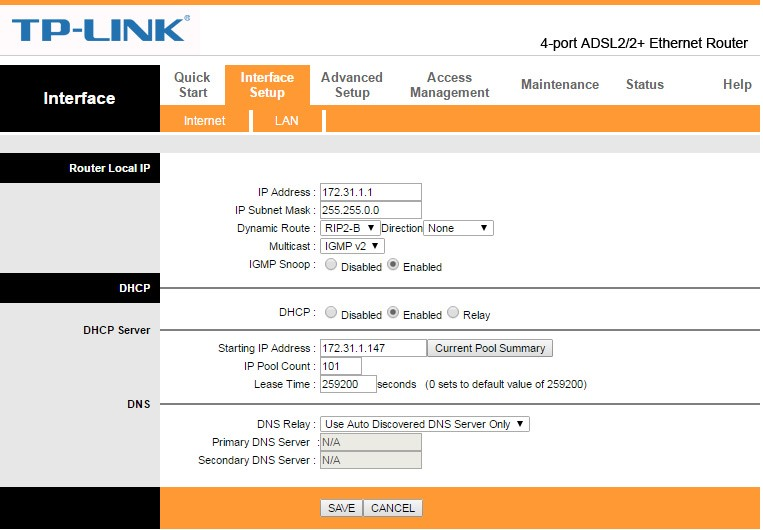
\includegraphics[width=0.9\textwidth]{network1}
				\end{center}
				
		
				
				\item After changing these values, the IP address used to access the router settings will change from (192.168.1.1) to the set gateway value (172.31.1.1) but with the same user name and password.
				
				fig6
				
				\begin{center}
					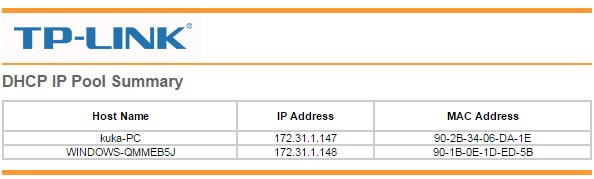
\includegraphics[width=0.7\textwidth]{network2}
				\end{center}
				
				\item The connection is now established and can be verified by checking the router LEDs
			\end{enumerate}
		
	\newpage
	\section{Installation of KUKA.Sim Pro}
	KUKA.Sim Pro is used for the complete offline programming of KUKA robots. This product allows the analysis of cycle times and the generation of robot programs. It also enables a real-time connection to the virtual KUKA robot controller (KUKA.OfficeLite). KUKA.Sim Pro is additionally used for building parametric components and defining kinematic systems, which can also be used in KUKA.Sim Layout and KUKA.Sim Tech. KUKA.OfficeLite is included in the KUKA.Sim Pro package. CAD importers are available as an option. This requires a purchasable license for each import interface. 
	


	\begin{center}
        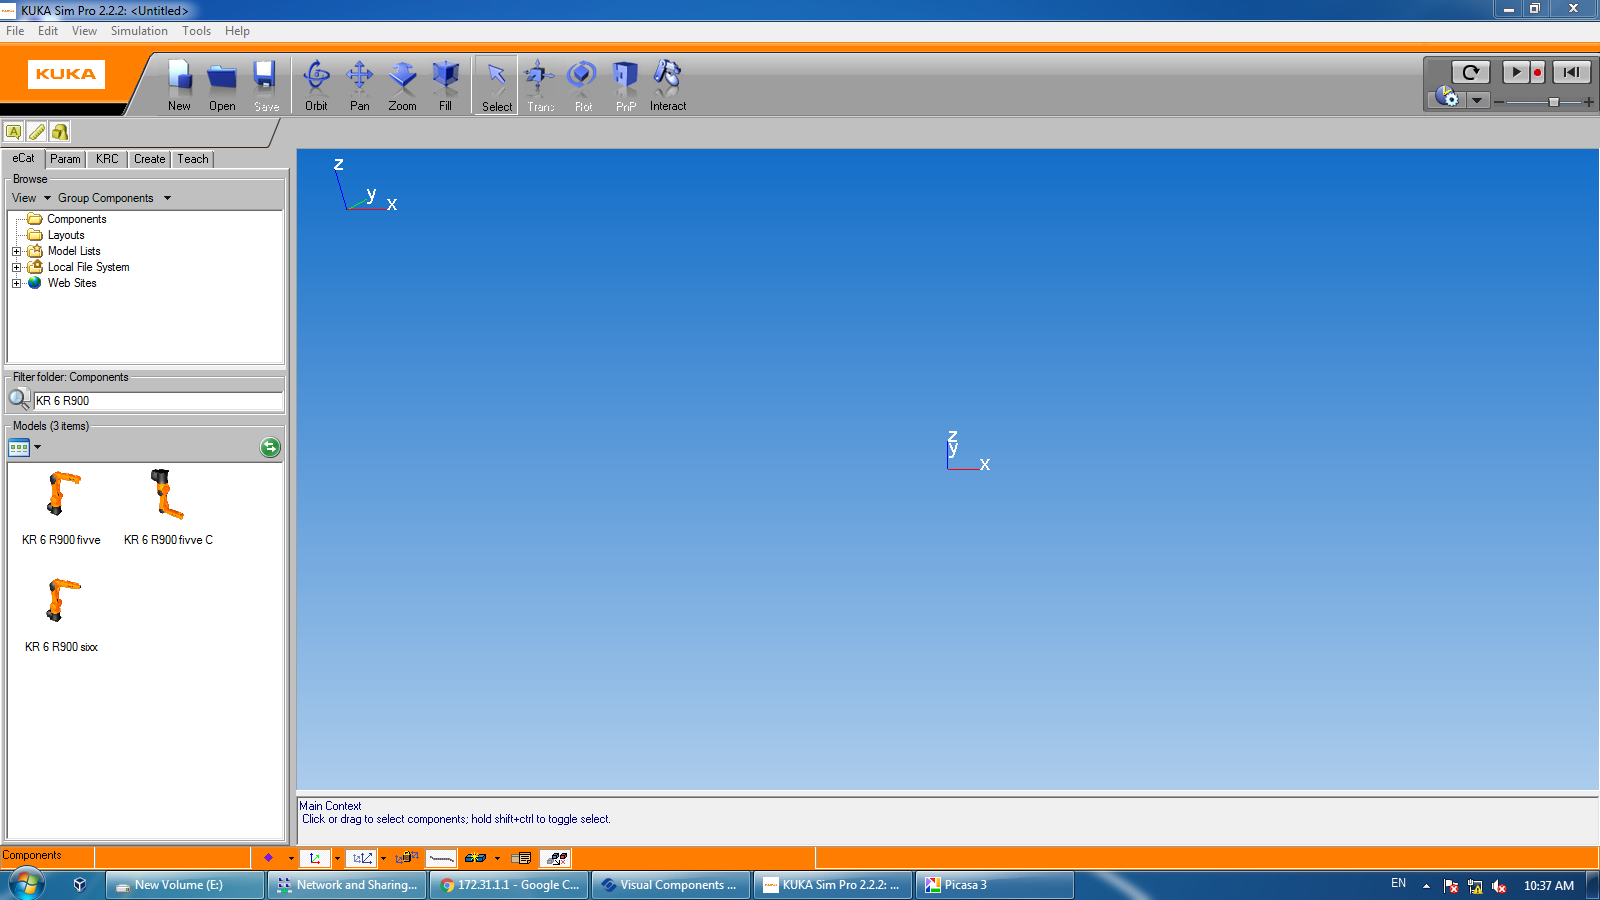
\includegraphics[width=0.9\textwidth]{simpro1}
	\end{center}
	 
	 \paragraph{Requirements}
	 	\begin{itemize}
	 	\item The minimum requirements for the computer are a 2 GHz CPU and 2 GB RAM, and an OpenGL-capable graphics card with at least 512 MB RAM and a resolution of 1024 x 768 pixels or a similarly specified notebook.
	 	\item Supported operating systems are WIN XP - 32-bit or WIN 7 - 32/64-bit.
	 \end{itemize}
 
 	\subsection{Installation}
 		\begin{enumerate}
 			\item Start the setup file “.exe”
 			\item Read the agreement and activate the check box “I accept ...”
 			\item Select “Install” to start installation.
 			\item Select “Install” to complete installation
 		\end{enumerate}
 	
 	\paragraph{Installing the component library }
 	After installation of the KUKA.Sim software product, the component library is installed with the following program: SetupKUKASimLibrary\_2.2.0\_Buildx.exe The procedure is very similar to the installation of the software products. Simply follow the instructions given.
 	The KUKA.Sim component library contains over 1,000 typical layout components (robots, grippers, fences, etc.), various demo layouts and tutorials for KUKA.Sim. Although the KUKA.Sim products still work without the component library installed, it is strongly recommended that the component library is installed in order to be able to create layouts quickly and easily.
 	
 	\subsection{License types}
 	There are different types of licensing for the KUKA software. License types are determined and verified in accordance with the purchase made from KUKA Roboter GmbH. 
 	The software licensing concerning the KUKA arm at Zagazig university is an educational bundle license. The serial number for the license is found in the booklet of the KUKA.Sim Pro CD. Information about different licensing bundles are obtained by contacting KUKA Roboter GmbH by email
 	\textbf {simulation@kuka-roboter.de.}
 	Further details about the steps of obtaining the serial key, for different commercial bundles,  are found on page 13 of (KUKA.Sim 2.2- Installation-en) manual.
 	The serial number associated with this purchase is: \textbf {K5P22-N174H-AW7KY-9}
 	
 		\subsubsection{Stand-alone License}
 		The license is on the PC on which KUKA.Sim is used. The license key is then valid for this PC only. It can also be transferred to a different PC, but cannot be used on a two different PCs at the same time, or when either of the two PCs is off.
 		
 		\subsubsection{Network License}
 		Network licenses provide a flexible way of using KUKA.Sim on more than one PC. When a license is requested by a PC, this license is then allocated to this PC. When KUKA.Sim is closed, the license becomes available again and can be accessed by other PCs. 
 		A license server is required to manage the network licenses. When KUKA.Sim Pro is started, the computer’s identity (IP address, please refer to \textbf {LAN connection} in manual Section “WorkVisual \& LAN connection”) is required occasionally, however, KUKA.Sim Pro needs to check with the local license server to make sure that KUKA.Sim Pro and server are on the same PC, which is required in the network license configuration.
 	
 				\paragraph{Requesting a license file manually}
 					\begin{enumerate}
 						\item Start the installation of KUKA.Sim Pro 
 						\item Enter the license key
 						\item Select “Activate manually” and save the request file
 						\item Go to the Visual components customer portal and use the given email and password, mentioned in the previous section, to login.
 						\item On the website, choose Manual Licensing, upload the request file and confirm.
 						
 						\begin{center}
                 	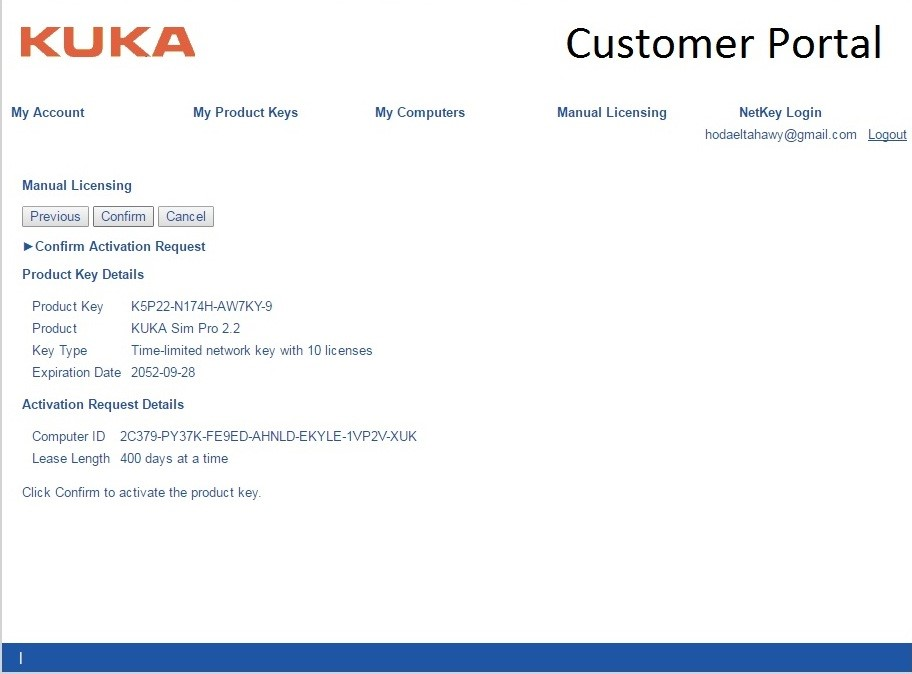
\includegraphics[width=0.9\textwidth]{simpro2}
 						\end{center}
 					
 					
 						
 						\item The license should be activated.
 						\item Download the license (.dat) file and click Finish. Please complete the installation steps of the license server before proceeding with the next steps.
 						\item The license (.dat) file should be loaded into the license server, not the KUKA.Sim Pro interface, in order to complete the activation process. 
                         \begin{center}
                 	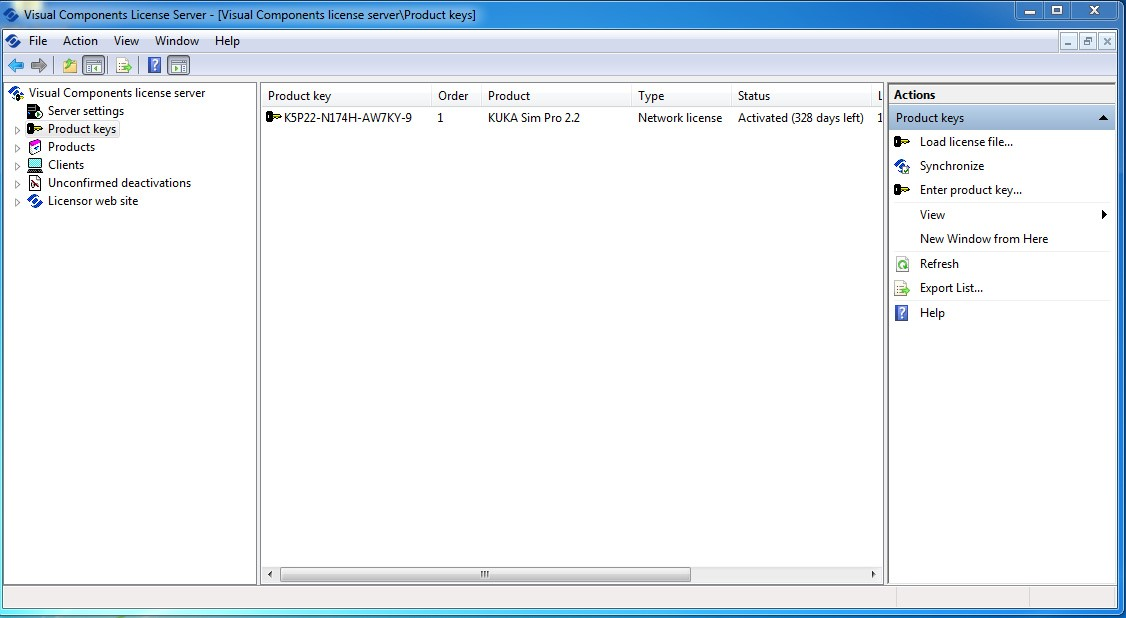
\includegraphics[width=0.9\textwidth]{simpro3}
                         \end{center}

 						\item After this process is completed, the network server interface should appear as follows
 					\end{enumerate}
 				
 				\paragraph{Installing the license server}
 				\paragraph{Requirements}
 				“Microsoft Management Console” (MMC) must be installed on the license server. The software can be downloaded from the Microsoft website. In addition, “.NET framework 3.5” or higher should be installed. 
 				
 				\paragraph{Installation}
 					\begin{enumerate}
 						\item The license server is started via “Start > Programs > Visual Components > Visual Components License Server > Visual Components License Server Manager”.
 						\item Choose “Server settings” from the left panel, make sure that the license server is started, if not, click Start to activate it. The port number value is 5093.
 						\item On the left-hand side, select “Product keys” in order to enter the license key.
 							\begin{itemize}
 								\item The right-hand side changes and “Enter product key...” is offered. Click on this.
 								\item A window is opened in the center, in which the license key can be entered.
 								\item If manual licensing is being performed using a license file, this license file must be loaded with “Load license file...”.
 							\end{itemize}
 						\item Enter the license key and confirm with OK.
 					\end{enumerate}
 				
 				For network licensing, an account linked with the purchase is created on the Visual Components website (http://www.visualcomponents.com/). In the specified customer portal (https://portal.visualcomponents.net/website/Login.aspx), sign in with the email hodaeltahawy@gmail.com and password quails@123 . In the “My Products keys” tab, you will find the product key for KUKA.Sim Pro on the KUKA-PC device, at the Mechatronics lab. The license is already activated and will only require renewal after a period of 400 days starting 3-12-2016, which is on 7-1-2018. 
	 
	 \newpage
	 \section{End-effectors installation}
	 	\subsection{Pneumatic gripper}
	 	The KUKA AGILUS offers numerous options for different end-effectors installations. One of the most common end effectors is a gripper, whether it be vacuum, pneumatic, hydraulic or servo-electric grippers. We are concerned with pneumatic grippers, which operate using air pressure. When air pressure is applied on the pistons, the gripper closes. When the pressure is released the gripper opens. The only way to manage the force in the gripper is to manage the air pressure in the air intake (or valve). The gripper used in our study is the SOMMER automatic GP 404 NC-C We also had the opportunity to work with one of KUKA Roboter’s Application software; Gripper\&SpotTech. These are ready-made software packages created for different industrial applications. Optional features can be installed on the controller easily and quickly and can also be tailored to the specific production environment. 
	 	
	 	These software include, and not limited to, KUKA.ArcTech, which enables implementation and programming of applications for arc welding and plasma cutting, KUKA.ConveyorTech, which automatically adapts the actions of the robot to the motion of an assembly line or conveyor belt and KUKA.CNC, which links the CNC and robot directly to each other. As a result, they can be operated like a conventional CNC controller.
	 	
	 	Pneumatic grippers can be used in many applications, some of which include assembly purposes, Labs automation, and on mobile robots.
	 	
	 	This software package offers numerous advantages, including:
	 		\begin{itemize}
	 			\item 16 freely configurable grippers
	 			\item 16 freely configurable grippers
	 			\item Gripper conditions statically and dynamically monitored
	 			\item Unlimited user-defined gripper icons
	 			\item Unlimited user-defined gripper icons
	 			\item Graphical user interface with indicator lamps, a status display and online adaptation
	 			\item Adaptation via WorkVisual 4.0 and on the smartPAD for production-relevant elements
	 		\end{itemize}
 		\newpage	
 		\subsubsection{Gripper connection}
 		The gripper is connected to the air supply through the Air 1 port located on link 3 (The port is shown in the following picture). This port is connected internally to Air 1 port on the back of the robot arm, which in turn is connected with the air compressor.
\begin{center}
    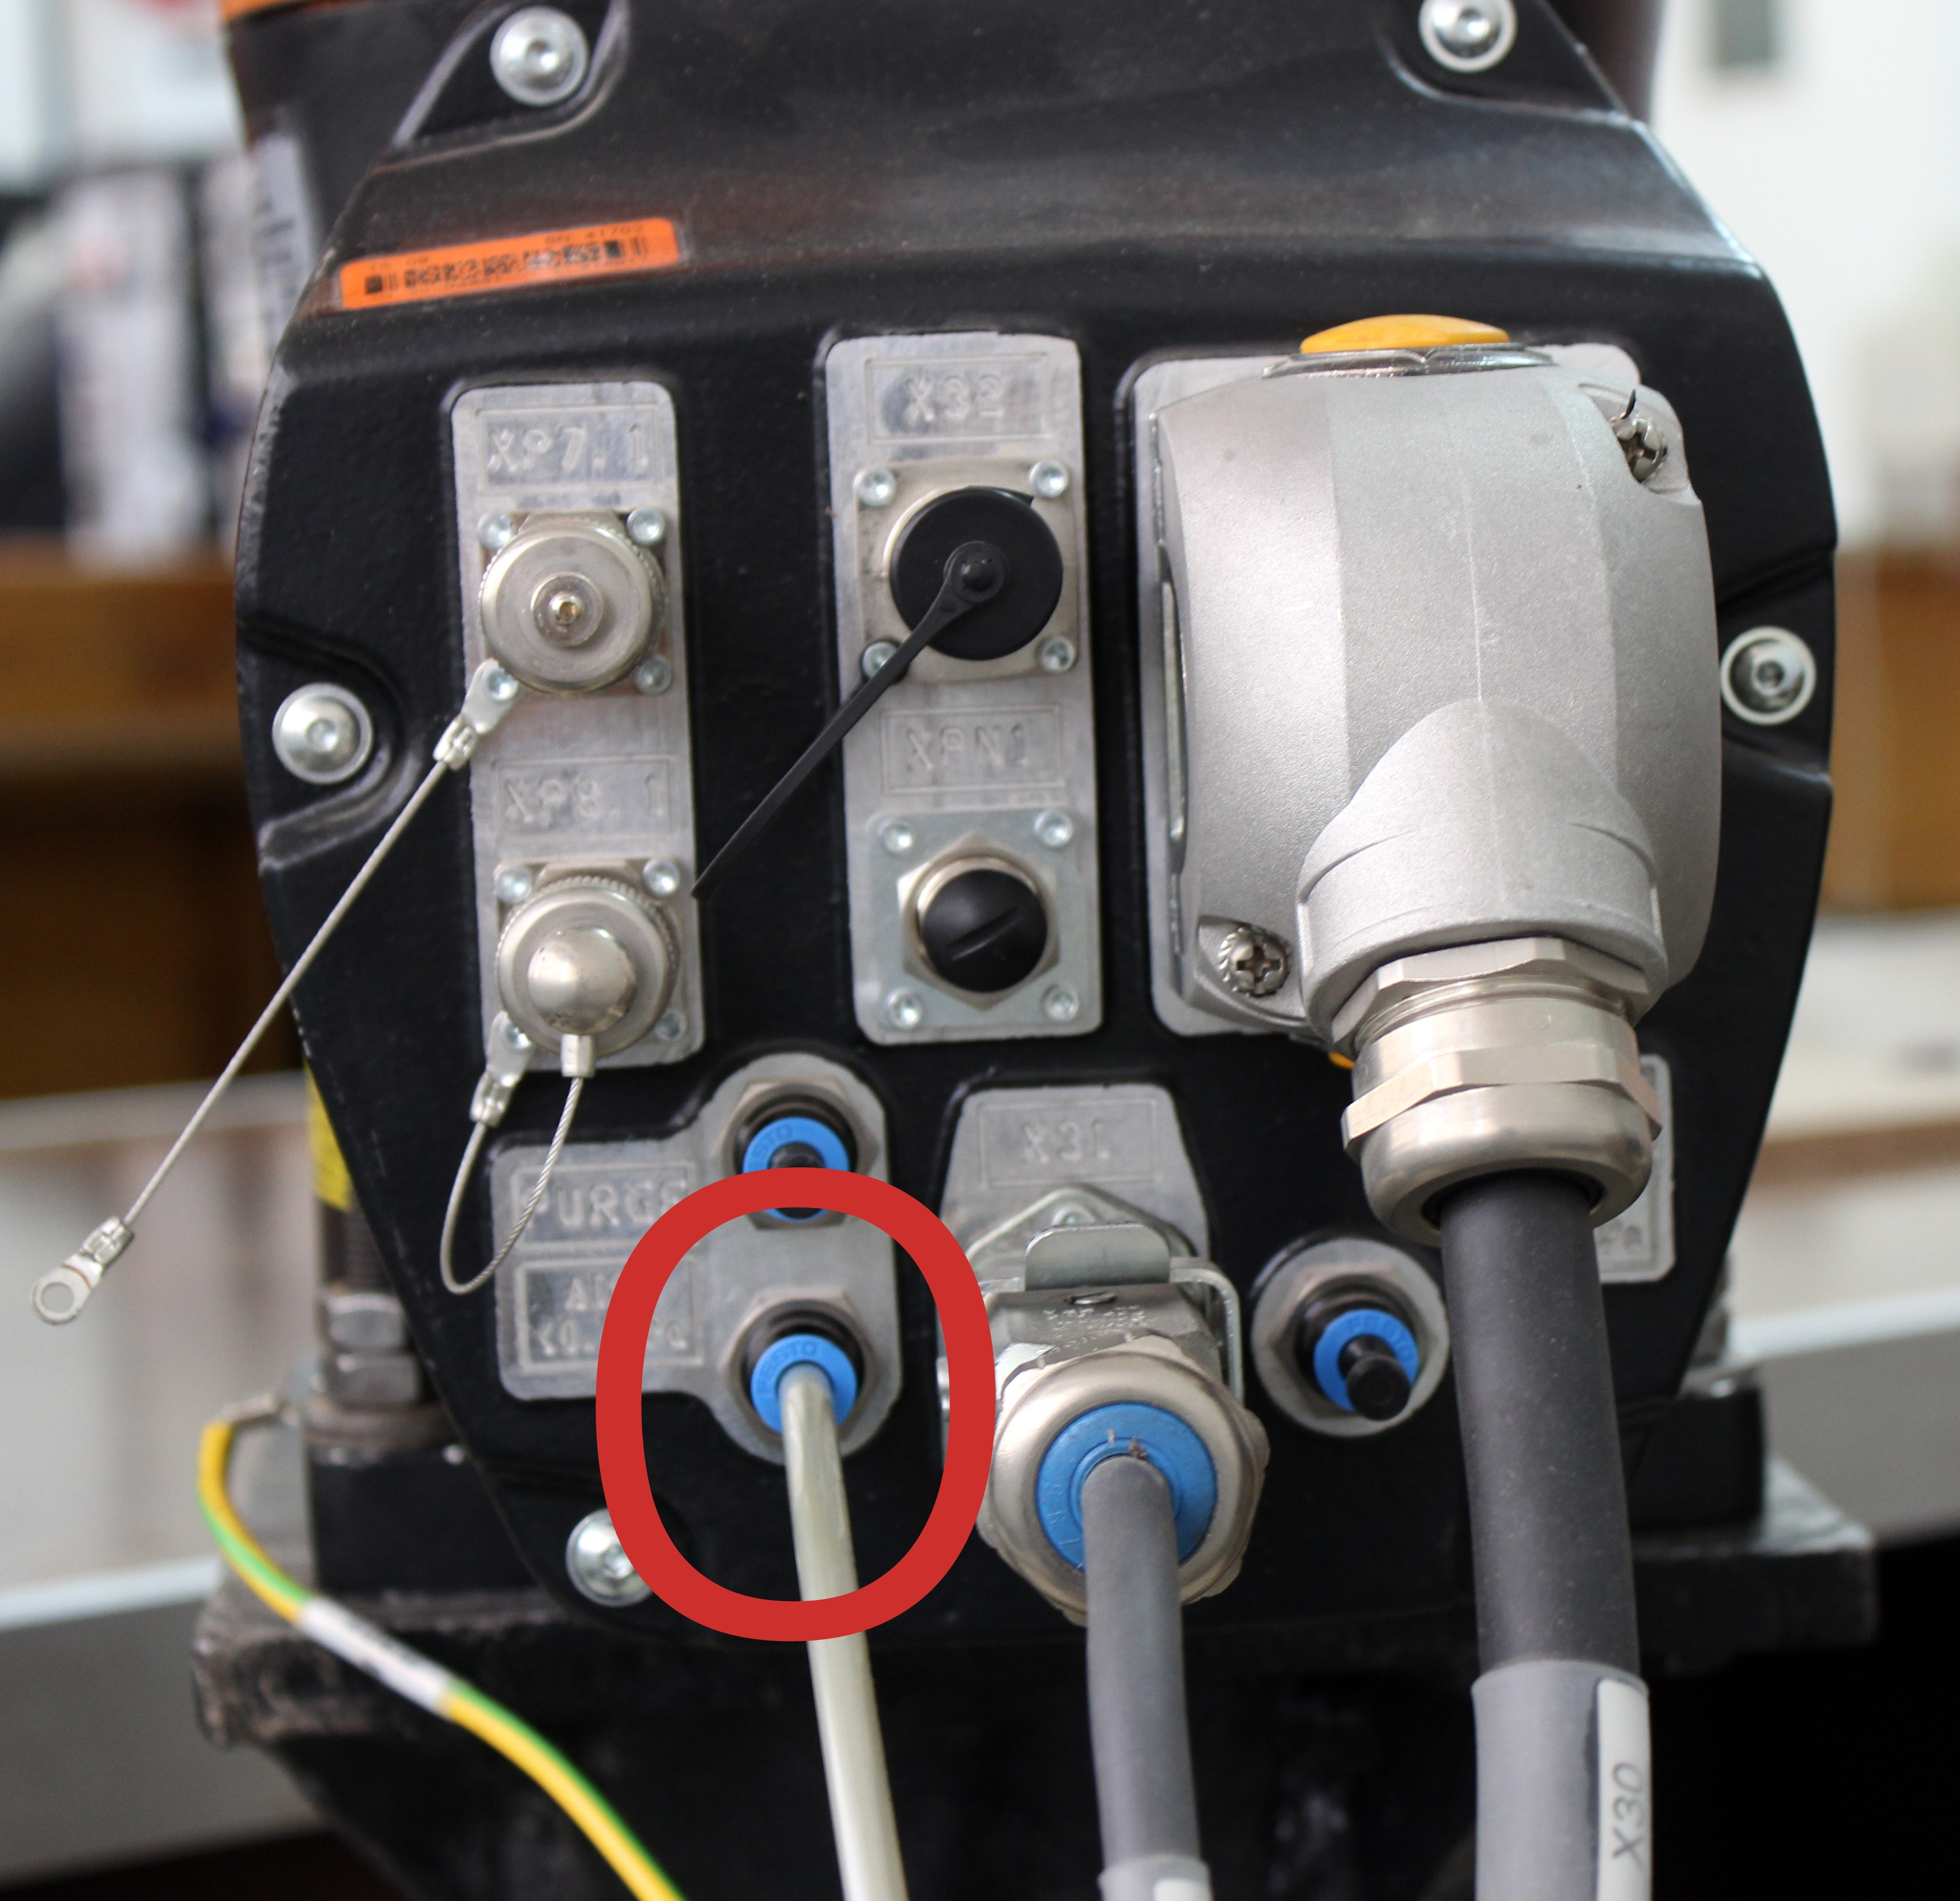
\includegraphics[width=0.45\textwidth]{gripper1}
    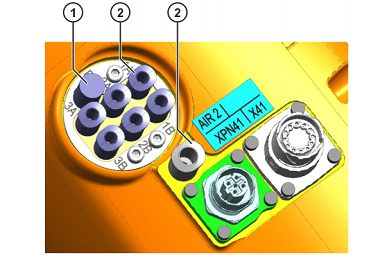
\includegraphics[width=0.5\textwidth]{gripper2}
\end{center}

 		\bigskip
 		In order for these ports to be operative, the connection between the ports and the controller must be activated, this is performed using mapping. Mapping can be simply described as the process of creating a link or a connection between ports on the robot arm and inner components in the controller in order to use them in control purposes, in our case operating the gripper. Mapping is performed through WorkVisual through the steps mentioned below.
 			\begin{enumerate}
 				\item get current project from robot using workvisual
 				\item save it as different file name
 				\item activate project in work visual (by double clicking on Controller<kss version>)
 				\item open I/O mapping
 				\item leave left pane on KRC (those are I/Os that robot programs can access), and click on inputs
 				\item move right pane to Fieldbus (those are physical I/O), then highlight EM8905 module (this is I/O card inside agilus arm)
 				\item map inputs of EM8905 to robot inputs of your choice
 				\item repeat steps 5.6.7 for outputs
 				\item on the robot login as Expert or higher (Expert will work in this case since we did not modify safety configuration)
 				\item deploy modified project to robot and activate it (on robot).
 				You should have something like on image below. 
 			\end{enumerate}
 		\begin{center}
 			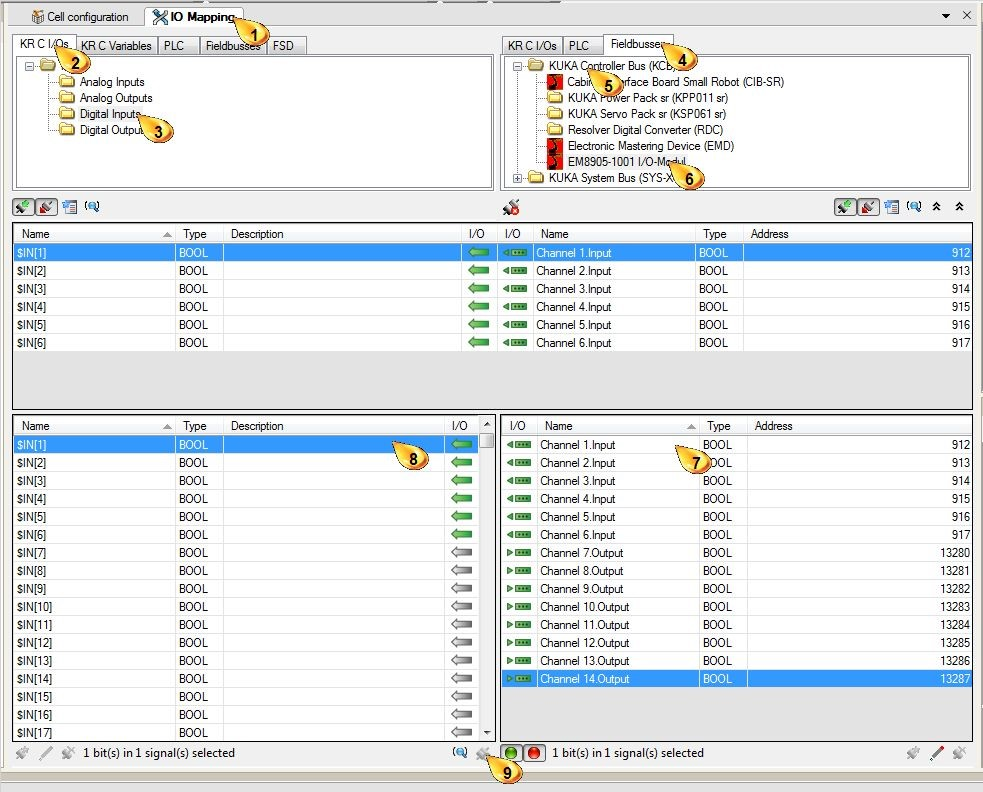
\includegraphics[scale=0.55]{gripper3}...
 		\end{center}
 	Six valves are mapped to ports:
 	\newline
 		\begin{minipage}{0.5\textwidth}
 			\begin{enumerate}
 				\item 1A
 				\item 2A
 				\item 3A
 				\item 1B
 				\item 2B
 				\item 3B
 				\item R (relief/exhaust) 
 			\end{enumerate}	
 	\end{minipage} \hfill
 	\begin{minipage}{0.5\textwidth}
 			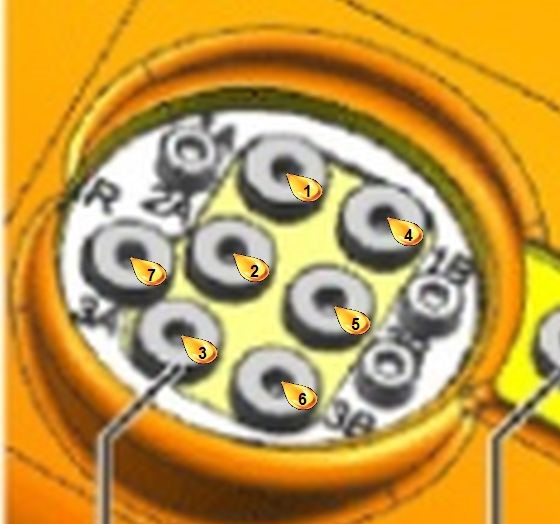
\includegraphics[scale=0.4]{gripper4}
 	\end{minipage}
 
 	\newpage
	\textbf{Configuring predefined grippers}

	\bigskip

	\begin{minipage}{0.5\textwidth}
	Gripper settings can be changed using smart pad. In the main menu, select Configure > I/O > Gripper. A window opens (shown in figure), inside it you’ll find a list of the predefined grippers, select the desired gripper number with Next or Previous. 
	\newline
	You can change number of grippers )1), Name of gripper (2), Type of gripper (3), designation of gripper type (4), Assignment of the output numbers (5), Assignment of the input numbers (6) and Switching states (7). 
	\newline
	The third cell, designated for the type of gripper is explained in the following section, Predefined gripper types.
	\end{minipage} \hfill
	\begin{minipage}{0.6\textwidth}
		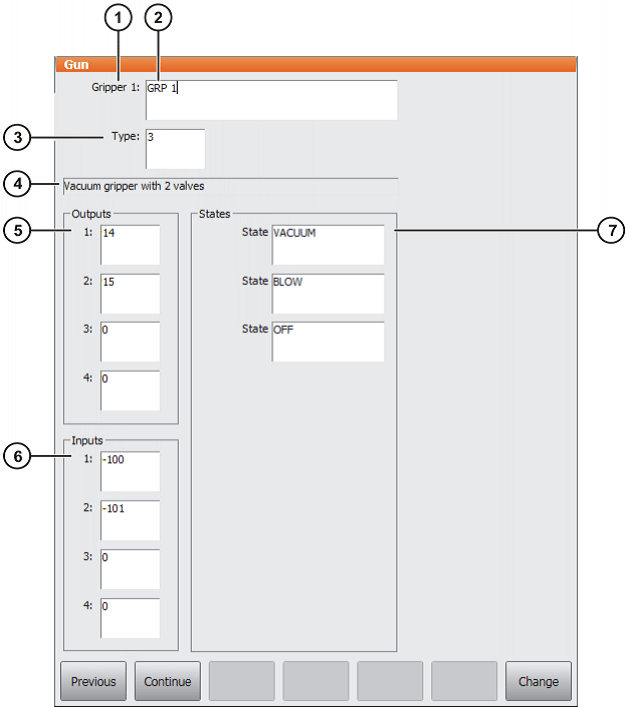
\includegraphics[scale=0.4]{gripper5}
	\end{minipage}
 		
 	\paragraph{Predefined gripper types}
 	There are five predefined gripper types in Gripper\&SpotTech. If these types are not sufficient, additional gripper functions can be programmed.
 		\begin{itemize}
 			\item Type 1: Single-element gripper, static, open/closed
 			\item Type 2: With mid-position valve
 			\item Type 3: Vacuum gripper with 2 valves
 			\item Type 4: Vacuum gripper with 3 valves
 			\item Type 5: Single-element gripper with pulse valves, open/close
 		\end{itemize}
 			\fbox{\begin{minipage}{32em}
 				More information about the specifications of each type and user specified grippers can be found in manual “KST\_GripperSpotTech\_32\_en”.
 			\end{minipage}
 		}

 		\paragraph{Gripper operation}
 		Manual gripper control can be performed using technology keys on smart pad. The settings for the technology keys are already set for this gripper and appear with the following icons on the smart pad screen, next to the assigned buttons. 
 		
 	\begin{center}
 		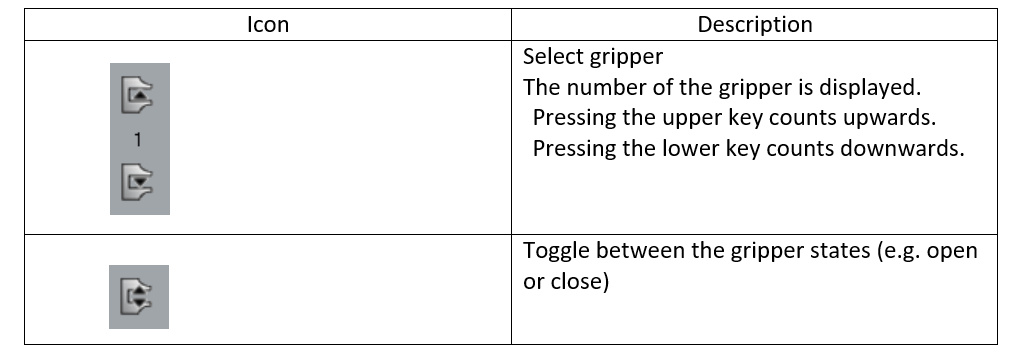
\includegraphics[scale=0.35]{gripper8} 
 	\end{center}
 
 The gripper is opened or closed using these buttons, after pressing the enable buttons on the back of the smart pad. They can also controlled inside KRL programs in inline form through the following command
 \begin{center}
 	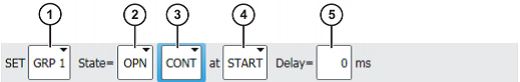
\includegraphics[scale=0.7]{gripper9}
 \end{center}
 
 	\paragraph{Where}
 	\begin{enumerate}
 		\item Choosing the desired gripper from a list of predefined grippers in settings
 		\item Set the state of the gripper, whether to open or close
 		\item CONT: Execution in the advance run
 		\item Box only available if CONT selected.
 			\begin{itemize}
 				\item START: The gripper action is executed at the start point of the motion.
 				\item END: The gripper action is executed at the end point of the motion.
 			\end{itemize}
 		\item Box only available if CONT selected.
 			Define a wait time (-200:200 ms), relative to the start or end point of the motion, for execution of the gripper action.
 		\item Box only available if [blank] selected.
 		Data set with gripper parameters
 	\end{enumerate}
 
 \subsection{Electric spindle}
 For the purpose of milling, a spindle was attached as an end effector to perform this process. The spindle used was a simple ON/OFF spindle, which required no control signals, so it merely needed to be attached to the end effector and to an external power supply. 
 
 \paragraph{Spindle attachment }
 For the spindle to be attached to the sixth axis of the robot, a metal linkage was designed and manufactured to fit both the spindle and the mounting surface on the sixth axis. The first picture shows the mounting surface of the sixth axis of the robot. The second shows the metal linkage after being installed to the mounting surface. The Third and fourth pictures shows the spindle’s metal holder. 
 
 \begin{center}
 	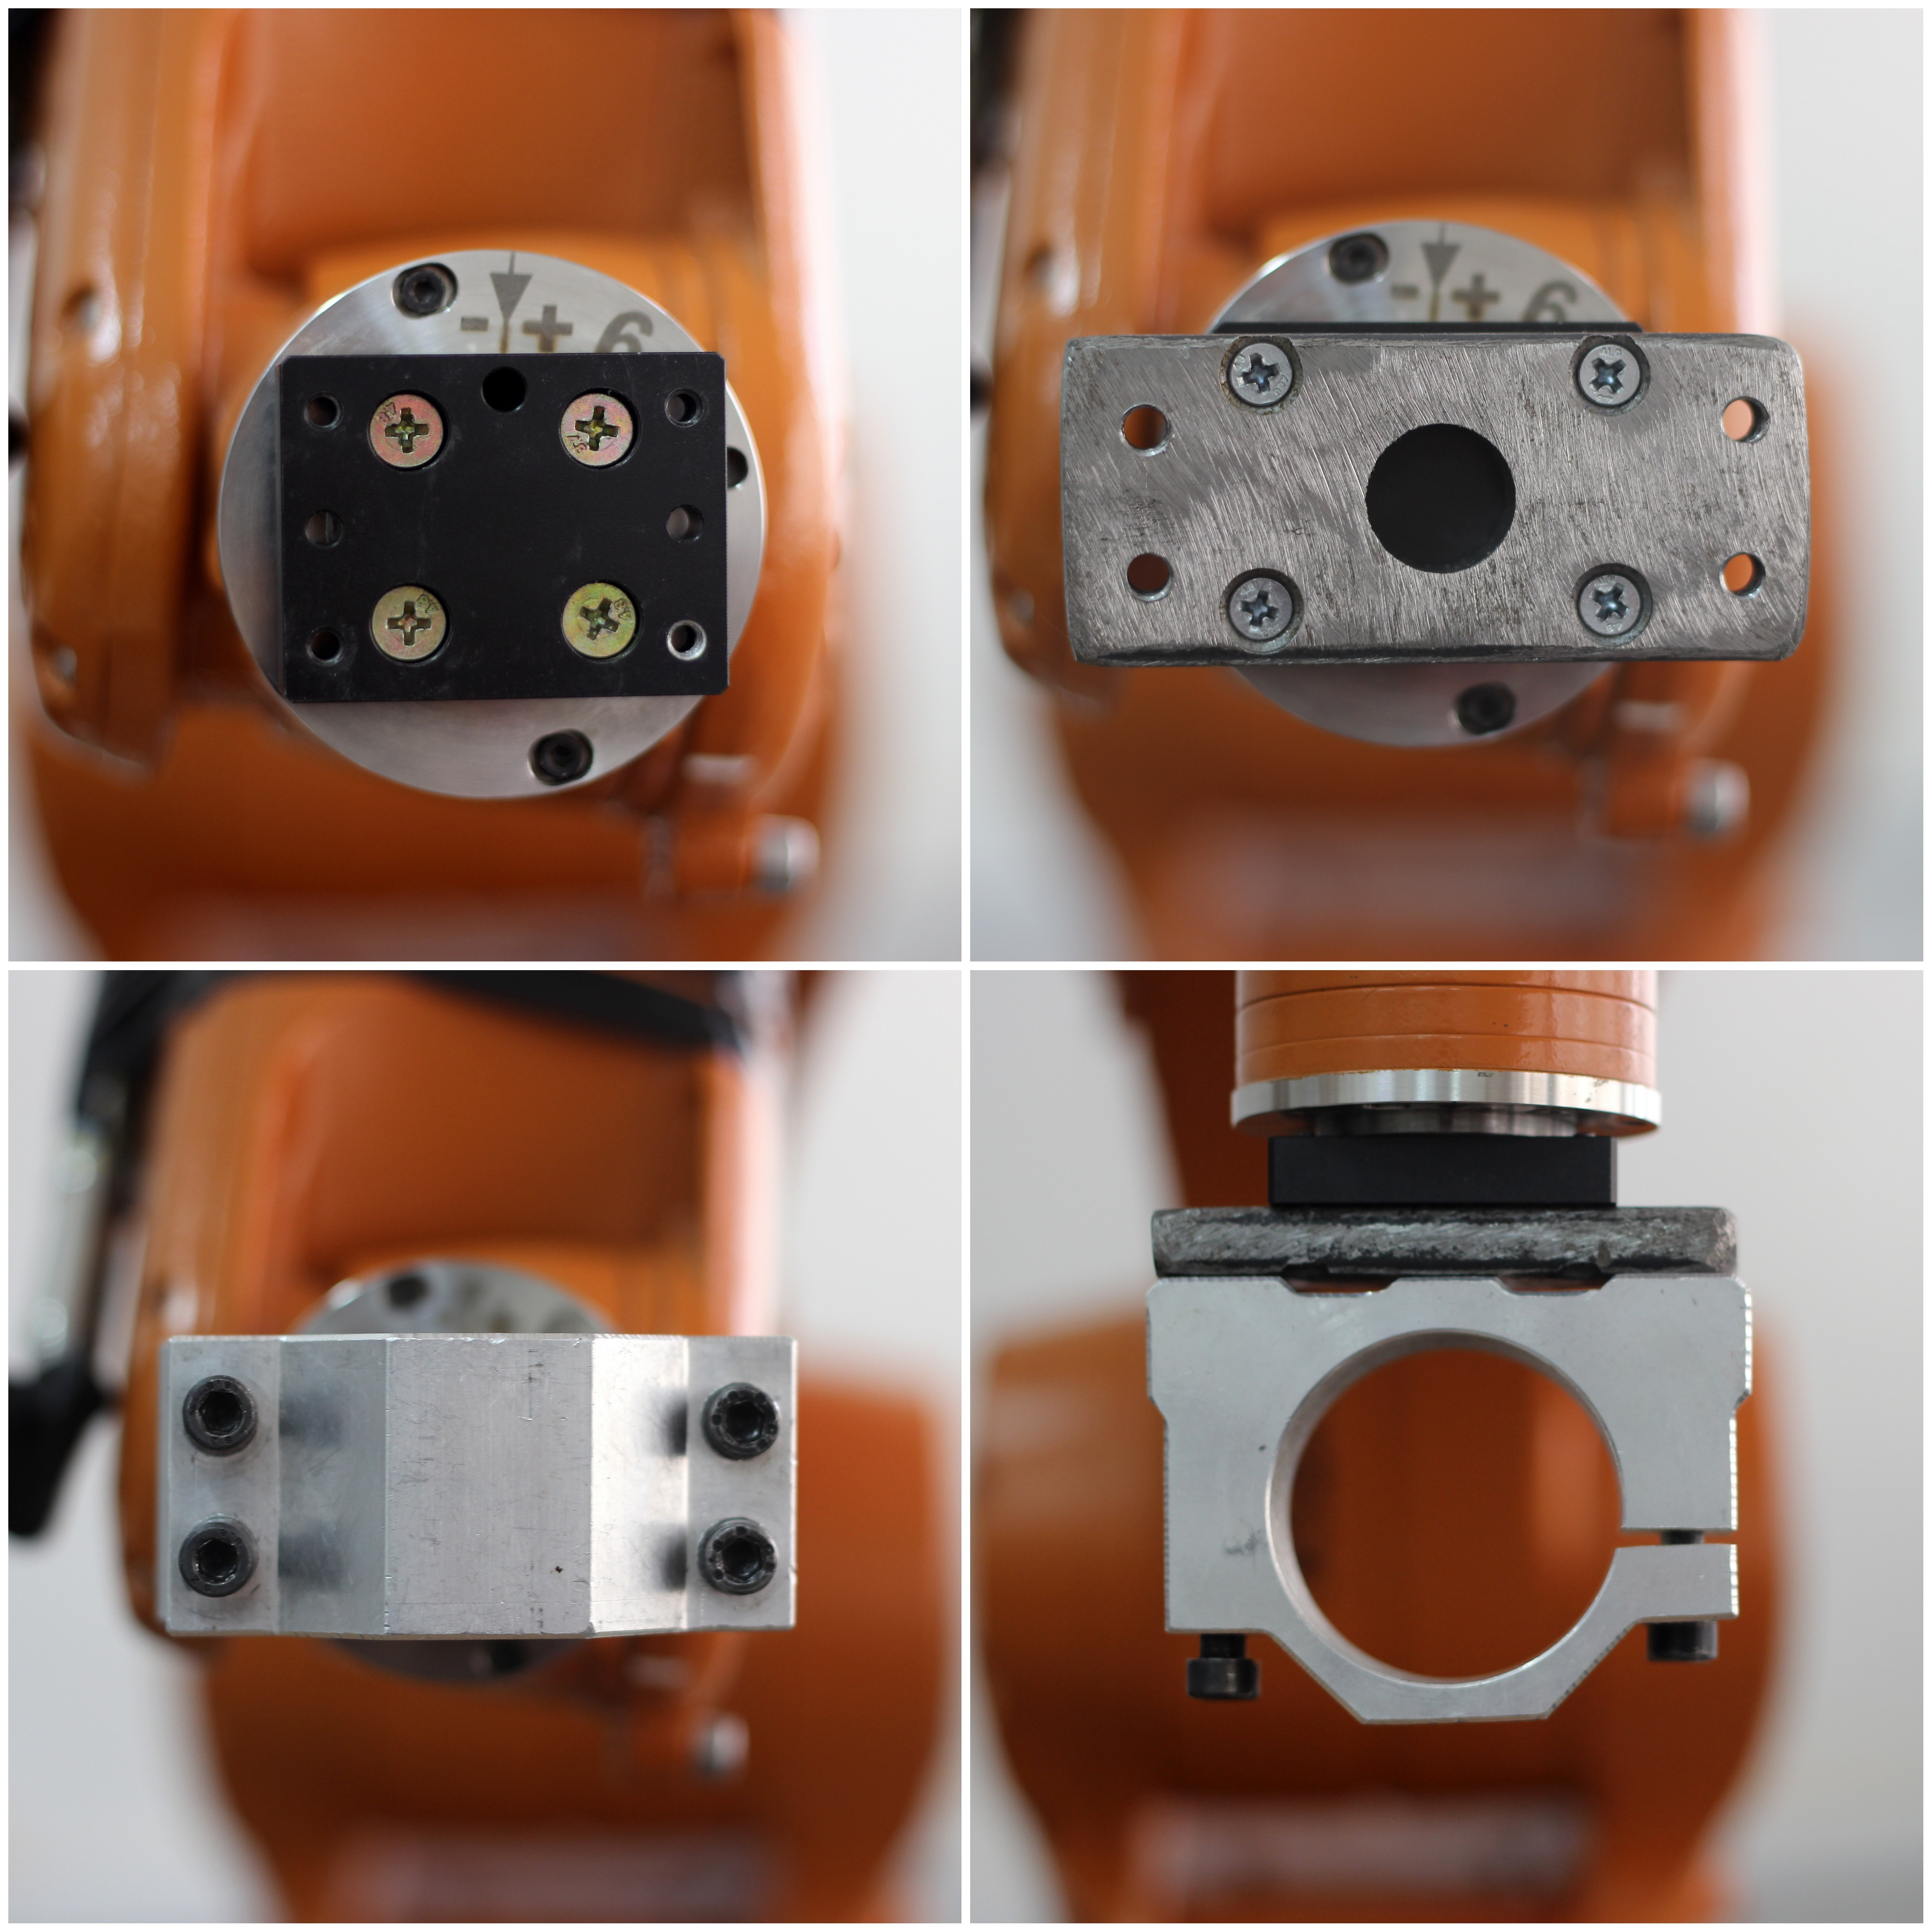
\includegraphics[scale=0.08]{spindle1}
 \end{center}

\paragraph{Spindle connection}
The power supply of the spindle is connected to port XPN1 on the fourth axis, whose output is internally linked to a similar port XPN1 on the back side of the robot. The port contains four openings or smaller ports; the positive wire is connected to the two right-hand side ports and the negative side to the left-hand side ports. The ports are shown in the picture below.

  \begin{center}
 	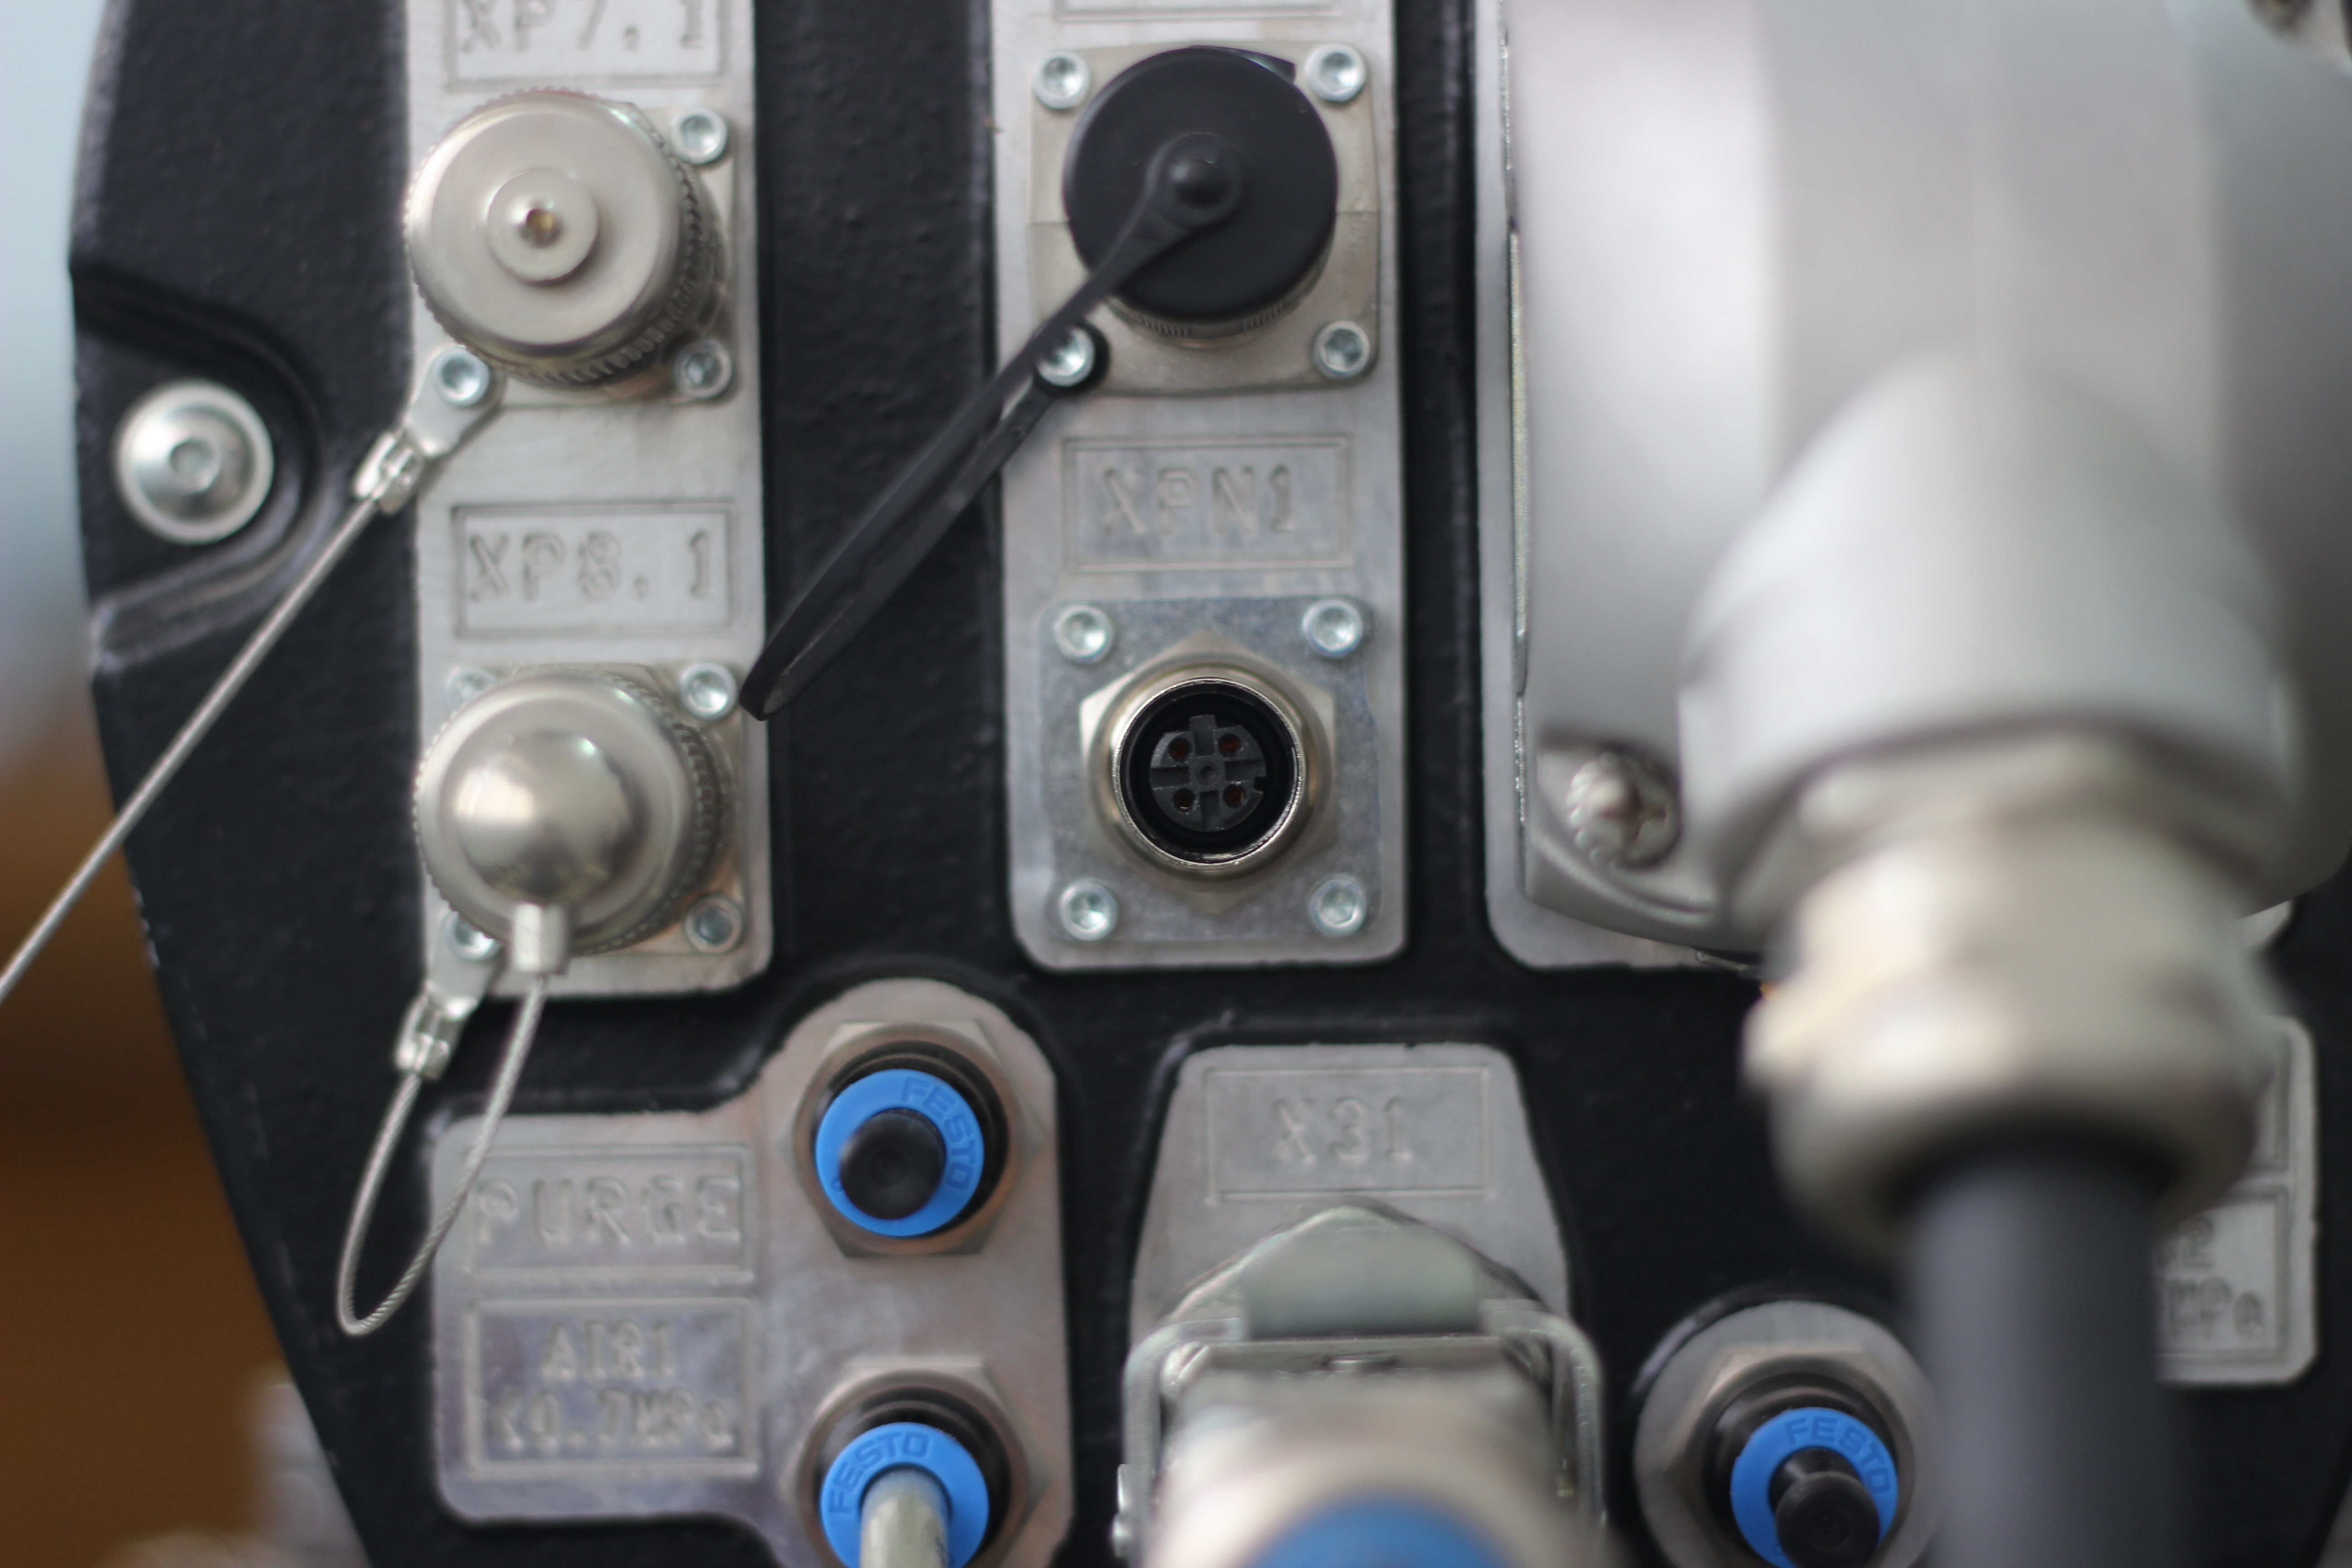
\includegraphics[scale=0.06]{spindle2}
 \end{center}

\paragraph{Spindle specifications }

The spindle used is an Air cooled spindle, with a 300W CNC Spindle Motor, supplied by a 220 voltage source, with adjustable speed through the attahced knob. The spindle must operate with full speed during the milling process. Further information about the spindle can be found in the resources in the references. 

\paragraph{End mill used for machining}

The end mill used is a double blade 6 mm Carbide blade. A 6 mm collet was used to attach the end mill to the spindle. A collet is a subtype of chuck that forms a collar around an object to be held and exerts a strong clamping force on the object when it is tightened, usually by means of a tapered outer collar. Both the end mill and the collet can be changed for different milling purposes, as an example, a smaller end mill can be used to obtain a higher level of fine details that larger end mills can’t offer, while larger end mills can be used to remove more material or perform faster in basic milling operations that does not require a high level of details.